
% *** BEGIN DOCUMENT ***
%
\begin{document}
\mode* % ignore text outside frames, useful to write notes



% *** FRAME #1 ***
%
% use:
%\frame[plain]{\titlepage}
% or:
\begin{frame}
~
\titlepage

\begin{center}

~

\includegraphics[scale = 0.9]{img/logo}
\vspace{0.5em} \\
\begin{minipage}{0.45\textwidth}
	\begin{flushleft} \large
		\emph{\tiny Author:}\\
		\textbf{Misha Mesarcik}\\
		\textit{\small msrmic004@myuct.ac.za}
		
	\end{flushleft}
\end{minipage}
~
\begin{minipage}{0.45\textwidth}
	\begin{flushright} \large
		\emph{\tiny :} \\
		\textbf{} \\
		\textit{\small }
	\end{flushright}
\end{minipage}\\[2cm]
\end{center}	
\end{frame}



%\begin{frame}{\huge Contents Page}
%	        \tableofcontents
%\end{frame}

\AtBeginSection[]
{
	\begin{frame}<beamer>
	\frametitle{Presentation Outline}
	\tableofcontents
\end{frame}
}


\section{Project Description}

\mode<all>{ 
	\SlideTransition{Project Description} 
}

\begin{frame}{\huge Introduction} 

 \begin{block}{Background to Study}<+->
 		\action<+->  {\begin{itemize}
			\item 	What is Digital Radio Frequency Memory? 
				\begin{itemize}
					\item[--] Digitize and store incoming RF input signals
					\item[--] Time delay 
					\item[--] Frequency shift
					\item[--] Scale Amplitude 
					\item[--] Retransmit
				\end{itemize}
				\item Used to deceive radars in ECM.
		\end{itemize}}
	\end{block} 
	\begin{block}{Motivations for Low Cost DRFM}<+->
		\action<+->  {\begin{itemize}
			\item DRFM systems are currently very expensive.
			\item Could be integrated into the PCL group's systems
		\end{itemize}}
	\end{block}
\end{frame}
\begin{frame}{\huge Introduction} 
\begin{block}{Archetypal DRFM Architecture}
	\action<+->  {\begin{figure}[h!]
			\centering
			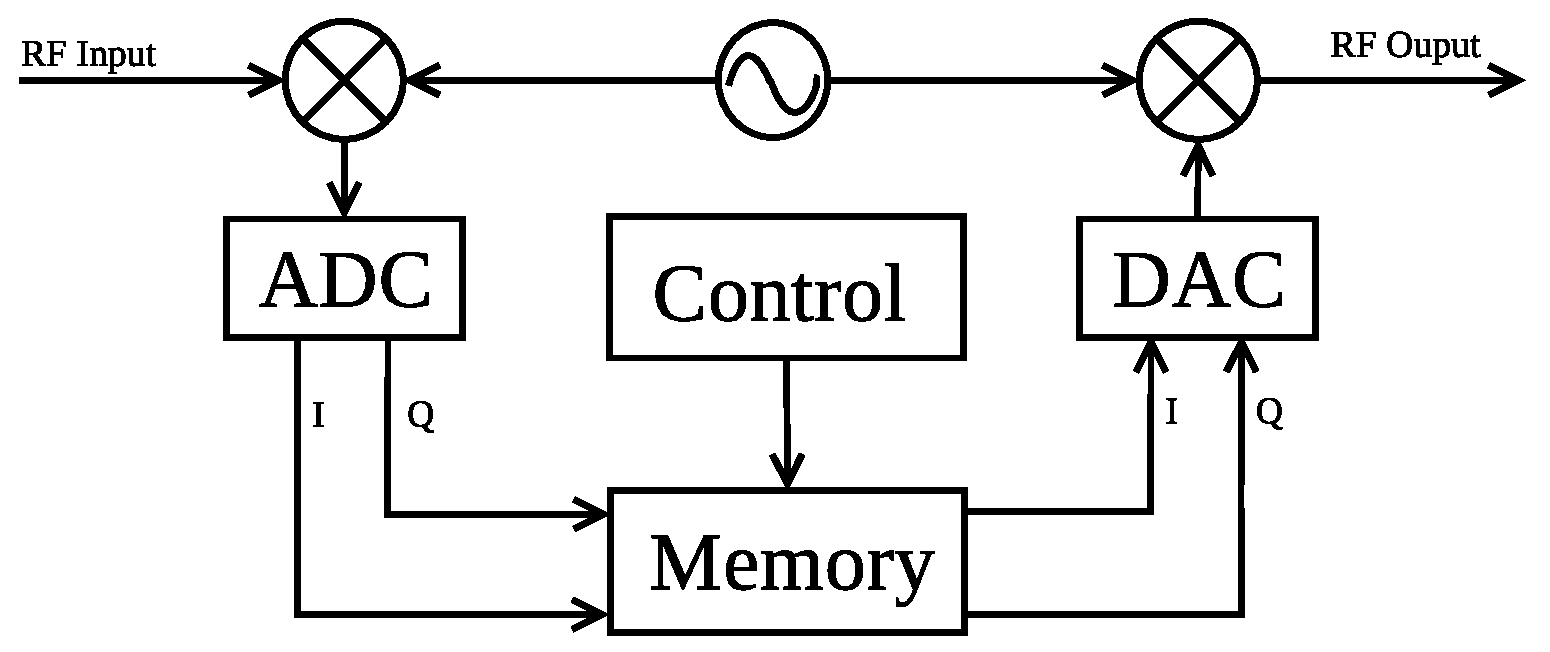
\includegraphics[scale = 0.43]{images/DRFM_Intro}
			\caption{DRFM Architecture}
	\end{figure}}
\end{block}
\end{frame}	



\mode<all>{ 
	\SlideTransition{System Overview} 
}

\section{System Overview}
\begin{frame}{\huge System Overview}
	\begin{block}{System break down}<+->
		\action<+->{
			On the FPGA there are the following subsystems
			\begin{itemize}
				\action<+->{\item Interfacing}
				\action<+->{\item Peripherals}
				\action<+->{\item Digital Signal Processing (DSP)}
			\end{itemize}
			}
	\end{block}
	
\end{frame}
\begin{frame}{\huge System Overview}
\begin{block}{System break down}<+->
	\action<+->{
		\begin{figure}[h!]
			\centering
			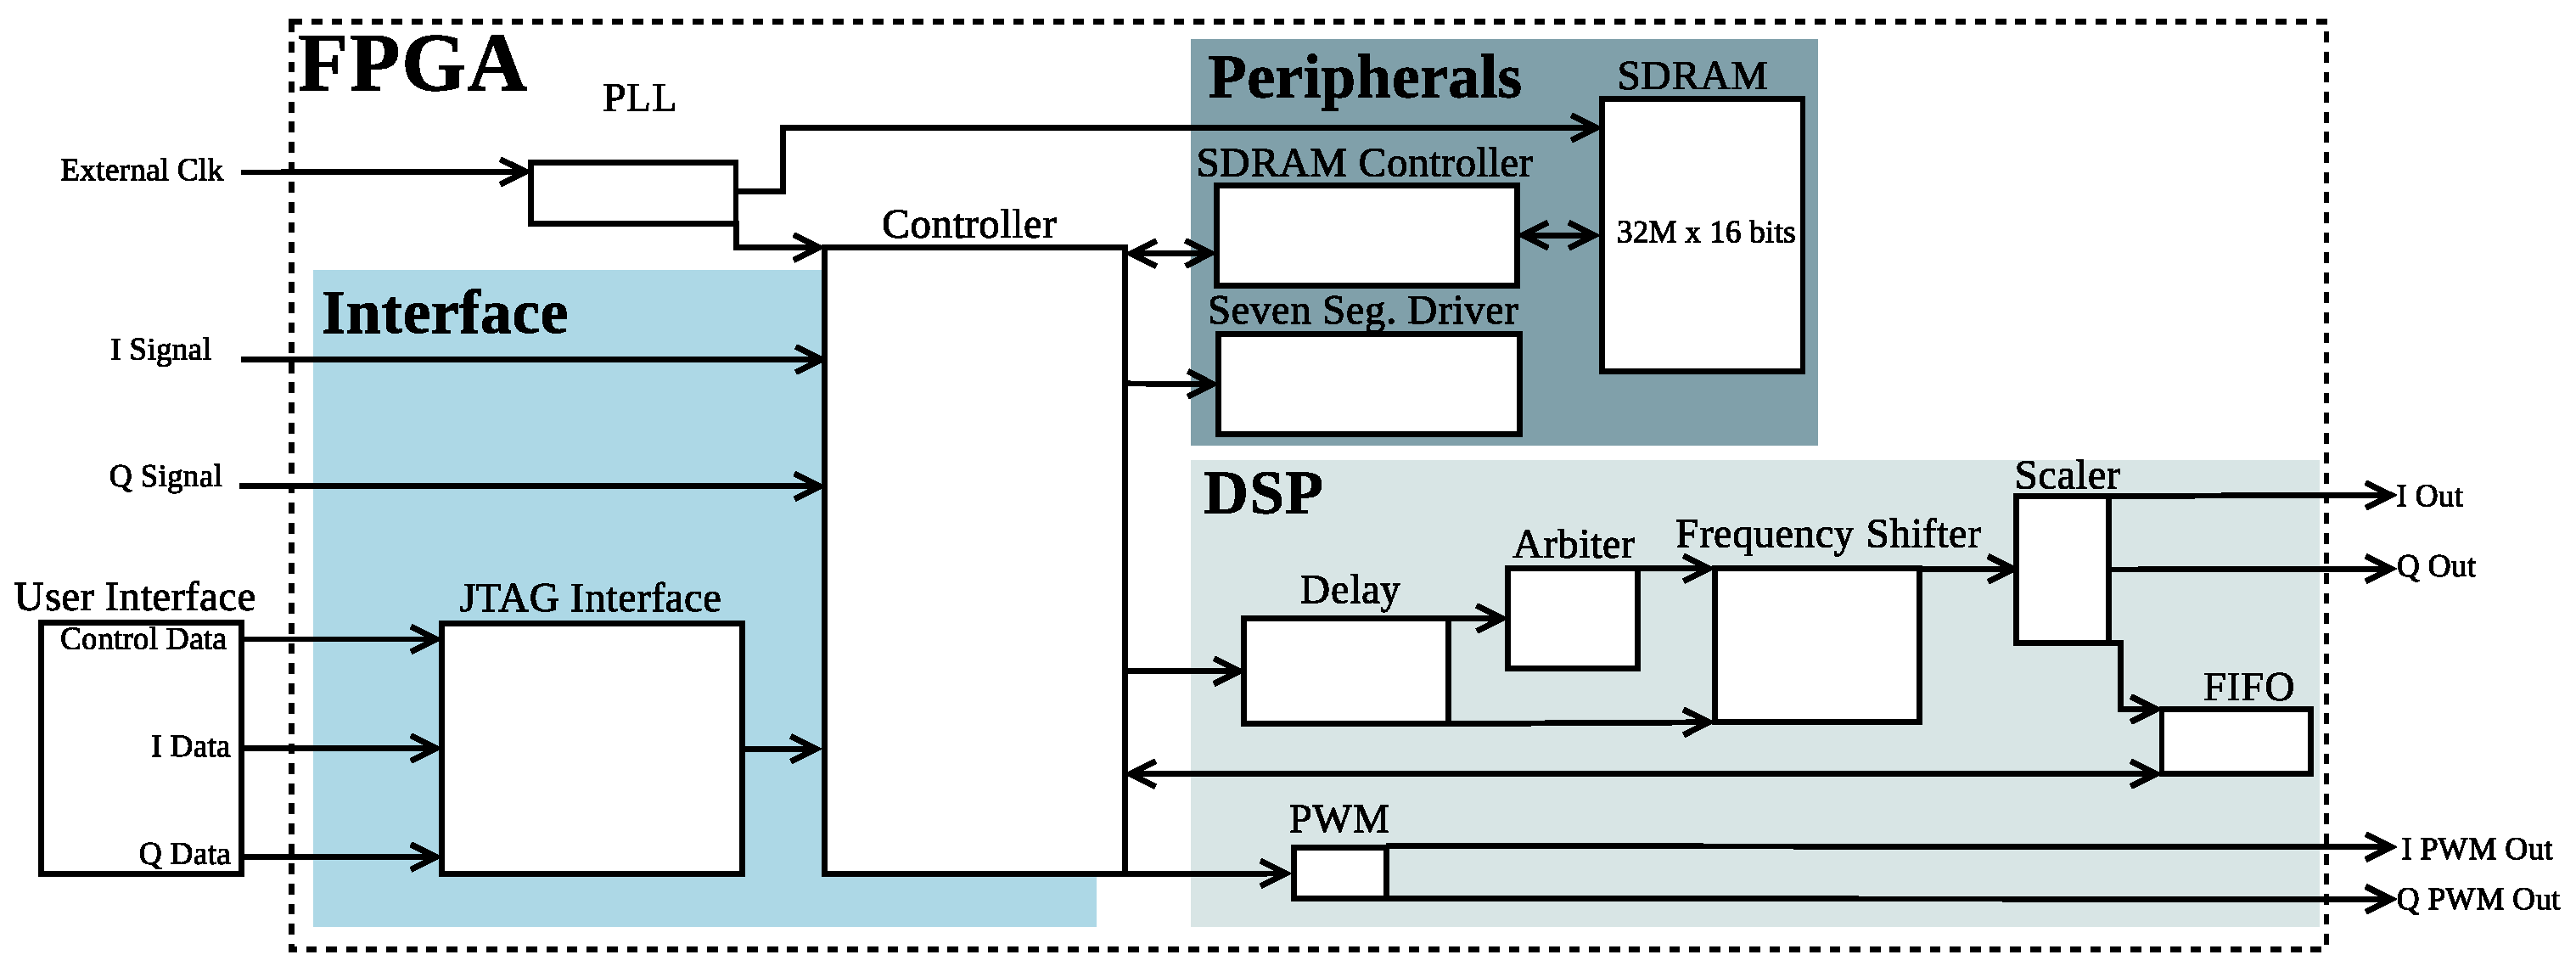
\includegraphics[width=\linewidth]{images/System_Overview}
			\caption{DRFM System Overview}
		\end{figure}
	}
\end{block}

\end{frame}




\begin{frame}{\huge System Overview}
	
	\begin{block}{JTAG Interface}<+->
		\action<+->{
		\begin{itemize}
			\item JTAG based interface
			\item Implements Altera's Virtual JTAG Interface IP Core
			\item Allows for both real time control and SDRAM Injection
			\end{itemize}}
	\end{block}
	\begin{block}{User Interface}<+->
		\action<+->{
		\begin{itemize}
			\item Built on PyQt and the Altera TCL scripting API
			\item Allowed for fine grain control over
			\begin{itemize}
				\item Frequency Shift (32 bit resolution)
				\item Time Delay      (10 bit resolution)
				\item Amplitude Scaling (16 bit resolution)
			\end{itemize}
			\item As well as facilitating I/Q Data injection into SDRAM
		\end{itemize}
	}
	\end{block}
		
\end{frame}


\begin{frame}{\huge System Overview} 
\begin{block}{User Interface }
	\action<+->  { \small	\begin{tabular}{ccc}
			
			\textbf{Control Information} & \textbf{Control Flag Position} & \textbf{Control Data Length} \\ 
			Doppler Shift 	& 33 & 32  \\
			Time Delay    	& 44 & 10 \\
			Amplitude Scale & 61 & 16 
		\end{tabular}
	}
\end{block}
\end{frame}	


\begin{frame}{\huge System Overview} 
	\begin{block}{External Peripherals}<+->
	\action<+->{
		\begin{itemize}
			\item Interfacing with SDRAM on the DE10-lite Development Board
			\item Seven Segment Display
			\item PWM output
		\end{itemize}
	}
\end{block}

\end{frame}

\begin{frame}{\huge System Overview} 
\begin{block}{Signal Model }<+->
	\action<+->{
		\begin{itemize}
			\item I/Q data was either received from RF front end or from SDRAM injection.
			\item Done to minimize sampling frequency criteria
			\item Both I and Q channels were 16 bits wide
		\end{itemize}	}
		\action<+->{\begin{equation*}
			s_{rx}(n) = v_{rx}(n) +j\hil \{v_{rx}(n)\} = I(n) +jQ(n)
		\end{equation*}}

\end{block}

\end{frame}

\begin{frame}{\huge System Overview} 
\begin{block}{Digital Signal Processing }<+->
	\action<+->{
		\begin{itemize}
			\item Order of operations was important
			\item Time Delay
			\begin{itemize}
				\item Worked by changing index of a RAM
				\item $	s_{delay}(k) = s_{rx}(n -k),\quad n \geq k$
			\end{itemize}
		\end{itemize}
	}
\end{block}

\end{frame}

\begin{frame}{\huge System Overview} 
\begin{block}{Digital Signal Processing }
		\begin{itemize}
			\item Frequency Shift
			\begin{itemize}
				\item As I/Q data was inject, it simplified the frequency shift operation
				\item Naturally a frequency shift is represented by a complex exponential representation: $	s_{s}(n) = s_{rx}(n) e^{j2\pi f_{s}n}$
				\item  Doesn't translate well to digital systems, so: 
				\begin{equation*}
				\label{eq:shift}
				\begin{split}
				s_{s}(n) &= [I(n) +jQ(n)][cos(2\pi f_{s}n) +jsin(2\pi f_{s}n)] \\
				&=  [I(n)cos(2\pi f_{s}n) - Q(n)sin(2\pi f_{s}n)] \\
				&\quad+j[I(n)sin(2\pi f_{s}n) +Q(n)cos(2\pi f_{s}n)]\\
				&= I_s(n) +jQ_s(n)
				\end{split}
				\end{equation*}
			\end{itemize}

		\end{itemize}
	
\end{block}
\end{frame}

\begin{frame}{\huge System Overview} 
	\begin{block}{Digital Signal Processing }
		\begin{itemize}
			\item Amplitude Scaling
			\begin{itemize}
				\item As UI sends a 16 bit amplitude control word need to somehow scale with it
				\item This value needs to be scaled so it is between 1 and close to zero 
				\begin{equation*}
					s_{scaled} (n) = 2^{-p} s_{rx}(n),\quad 0 \leq p \leq 15
				\end{equation*}
			\end{itemize}
		\end{itemize}
	
	\end{block}

\end{frame}

\mode<all>{ 
	\SlideTransition{Detailed Design} 
}
\section{Detailed Design}
\begin{frame}{Detailed Design}
		\begin{columns}
			\column{0.5\textwidth}
			\begin{block}{User Interface}<+->
				\action<+->{	\begin{itemize}
						\item Always be available to send control data
						\item Should be able to quickly change to SDRAM Injection
						\item Using PyQt/Altera TCL Scripting API
					\end{itemize}}
					\begin{table}[h!]
					\centering
					\caption{Control Word Composition}
									\label{tab:Control_Info}
				\end{table}
		
			\end{block}
			\column{0.5\textwidth}
			\begin{block}{UI Flowchart}<+->
				\action<+->{\begin{figure}[h!]
					\centering
					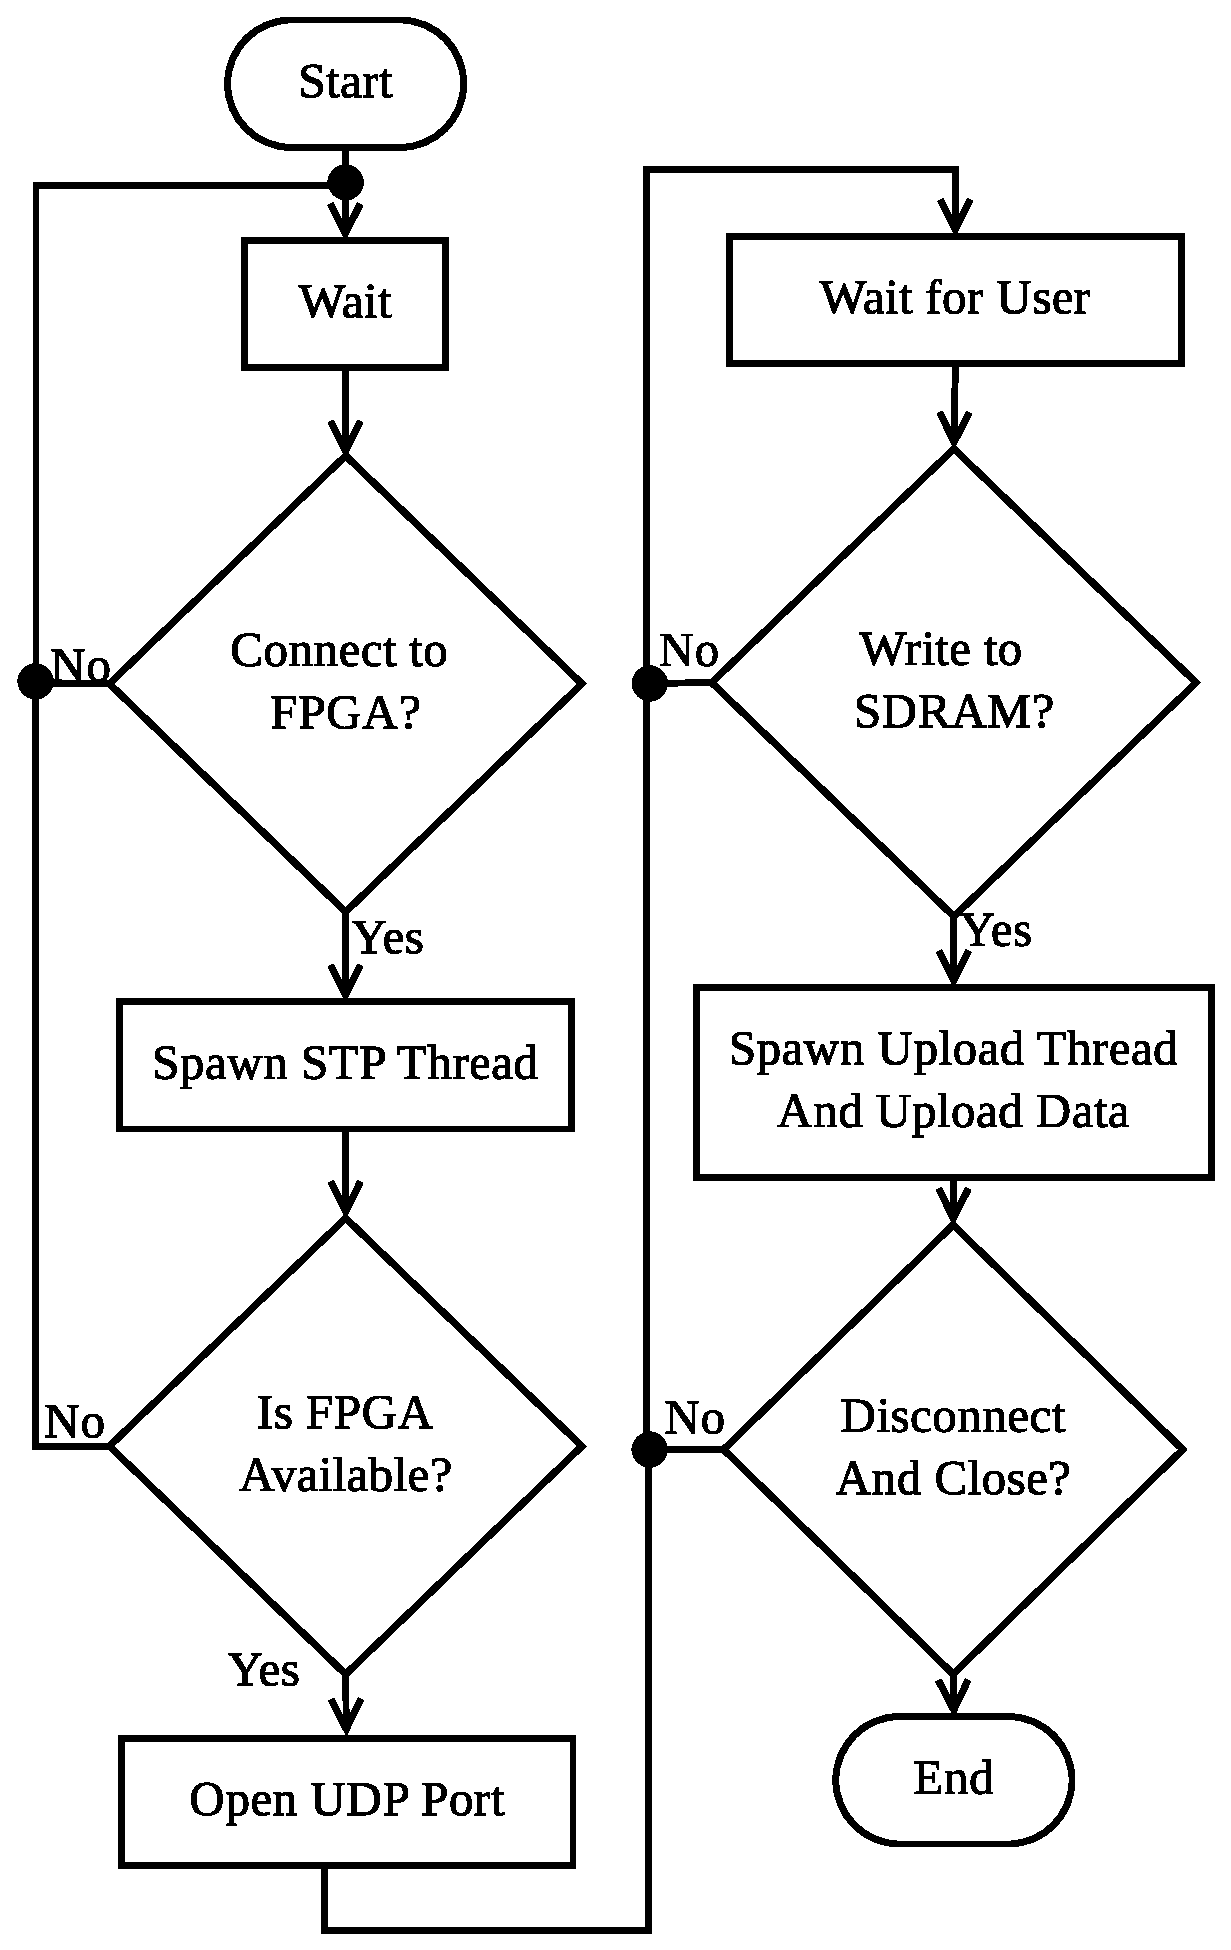
\includegraphics[width=0.6\linewidth]{images/UI_Flowchart}
					\caption{Flow chart showing the User Interfacing Structure}
				\end{figure}}
			\end{block}
		\end{columns}
\end{frame}

\begin{frame}{Detailed Design} 
\begin{block}{User Interface }
	\action<+->  {\begin{figure}[h!]
			\centering
			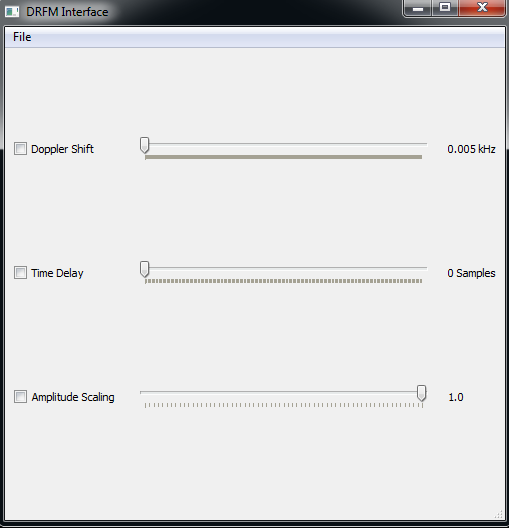
\includegraphics[scale = 0.43]{images/UI}
			\caption{Functional UI}
	\end{figure}}
\end{block}
\end{frame}	


\begin{frame}{Detailed Design}
\begin{columns}
	\column{0.5\textwidth}
	\begin{block}{JTAG Interface}<+->
		\action<+->{	\begin{itemize}
				\item Two modes of operation
				\begin{itemize}
					\item Write Data (TDI line routed to SDRAM Controller)
					\item Data Capture Mode (TDI line shifted and captured)
					\item Determined by UI and by SW0 on Development Board
				\end{itemize}
				
		\end{itemize}}
		
	\end{block}
	\column{0.5\textwidth}
	\begin{block}{JTAG Physical Lines}<+->
		\action<+->{\begin{figure}[h!]
				\centering
				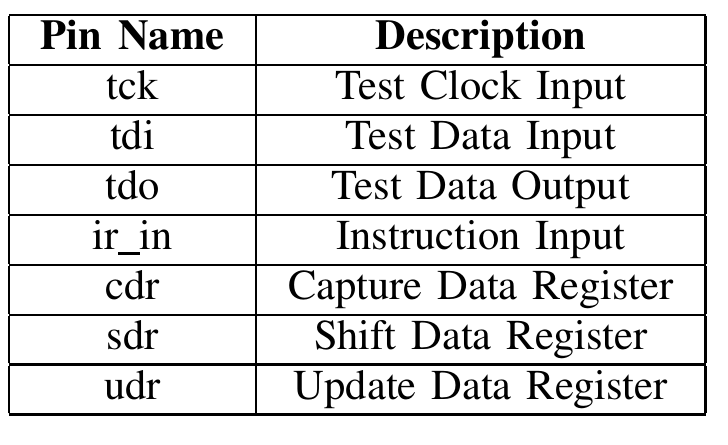
\includegraphics[width=0.6\linewidth]{images/tbl}
				\caption{Table showing JTAG lines used}
		\end{figure}}
	\end{block}
\end{columns}
\end{frame}


\begin{frame}{\huge Detailed Design} 
\begin{block}{Controller Module }
	\begin{itemize}
			\item Arbitrates between SDRAM and RAM 
			\begin{itemize}
				\item Dependant on \texttt{Read\_DataValid} and \texttt{Read\_WaitRequest}
			\end{itemize}
			\item Also performs changes in assignment for reading and writing from SDRAM
	\end{itemize}
	
\end{block}
\end{frame}

\begin{frame}{\huge Detailed Design} 
\begin{block}{SDRAM Subsystem}
	\begin{itemize}
		\item Uses Altera's SDRAM Controller IP Core
		\item Uses Altera's PLL IP Core
			\action<+->{\begin{figure}[h!]
				\centering
				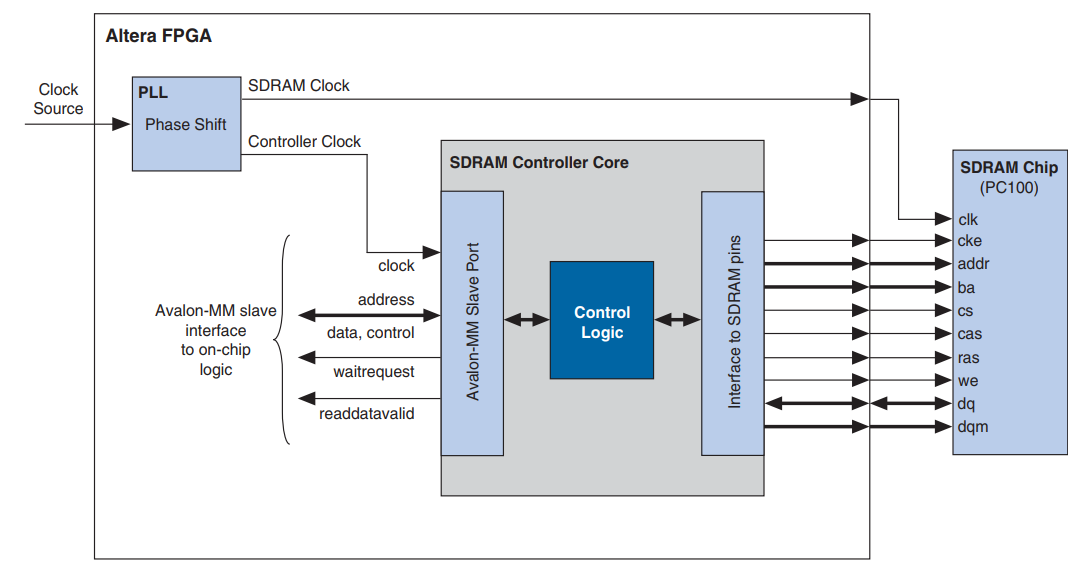
\includegraphics[width=0.9\linewidth]{images/SDRAM}
				\caption{Block Diagram of the SDRAM interfacing subsystem}
		\end{figure}}
	\end{itemize}
	
\end{block}
\end{frame}

\begin{frame}{\huge Detailed Design} 
\begin{block}{DSP Chain}
	\begin{itemize}
		\item Delay module
			\begin{itemize}
				\item Integrated into the controller module
				\item Takes data from SDRAM
				\item Writes it to a 2048 address wide RAM 
				\item Implements a state machine for keeping track of the indexing
			\end{itemize}
	\end{itemize}
	
\end{block}
\end{frame}

\begin{frame}{Detailed Design}
\begin{columns}
	\column{0.5\textwidth}
	\begin{block}{DSP Chain}<+->
		\action<+->{	\begin{itemize} 
				
				\item Arbiter
				\begin{itemize}
					\item As data in SDRAM was 16 bits per address
					\item Each I/Q were 16 bits wide each
					\item Needed both for Frequency shifting operation
					\item Used FSM to arbiter RAM data so that both I/Q data streams were available at the same time
				\end{itemize}
				
		\end{itemize}}
		
	\end{block}
	\column{0.5\textwidth}
	\begin{block}{Arbiter State machine }<+->
		\begin{figure}[h!]
			\centering
			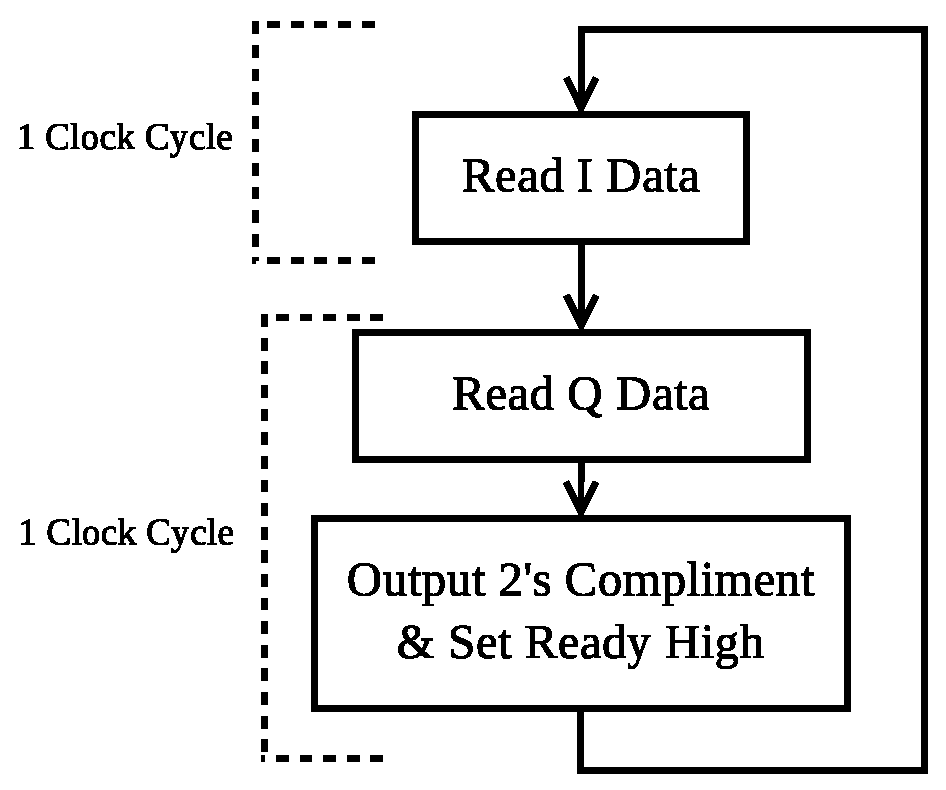
\includegraphics[width=0.9\linewidth]{images/Arbiter_State_Machine}
			\caption{State Diagram of the Arbiter}
		\end{figure}
	\end{block}
\end{columns}
\end{frame}

\begin{frame}{Detailed Design}
\begin{columns}
	\column{0.5\textwidth}
	\begin{block}{Frequency Shifter}<+->
		\action<+->{	\begin{itemize} 

						\item NCO
						\begin{itemize}
							\item Required to perform frequency shifting as per equation shown previously
							\item Look up table that translates input frequency to a periodic waveform
							\item Used a 4086 address dual port ram 
							\item Address counters were 1024 addresses out of phase to get both sine and cosine
							\item Initialized with MATLAB script  
						\end{itemize}

			\end{itemize}}
		
	\end{block}
	\column{0.5\textwidth}
	\begin{block}{NCO Block Diagram}<+->
		\begin{figure}[h!]
				\centering
				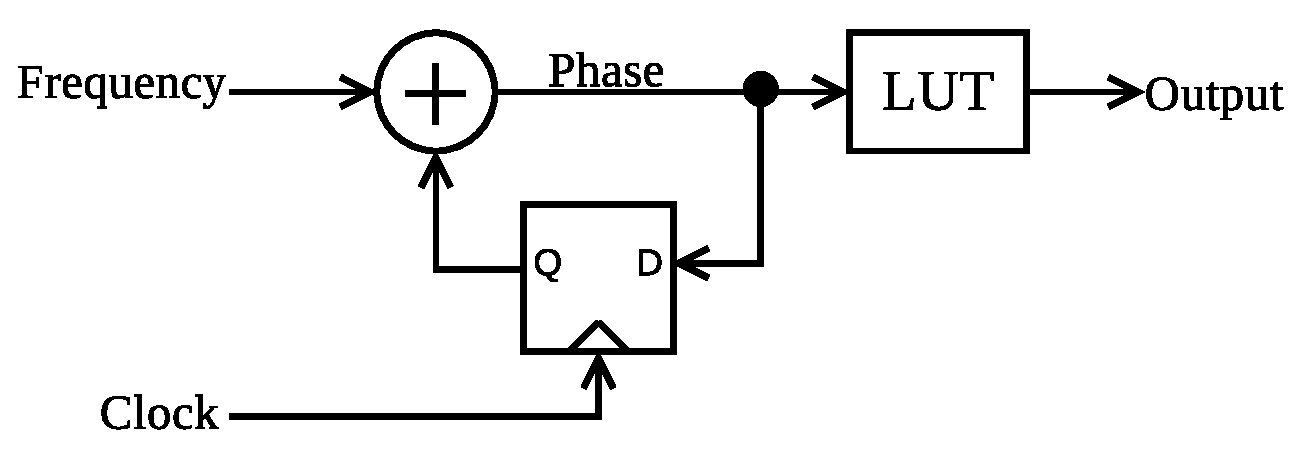
\includegraphics[width=0.9\linewidth]{images/NCO}
				\caption{Diagram of NCO Operation}
		\end{figure}
		\begin{equation*}
		f_{shift } = f_{slider} \dfrac{2^{32}}{100MHz}
		\end{equation*}
	\end{block}
\end{columns}
\end{frame}


\begin{frame}{Detailed Design}
\begin{columns}
	\column{0.5\textwidth}
	\begin{block}{Frequency Shifter}<+->
		\action<+->{	\begin{itemize} 
				
				\item Arithmetic Operations
				\begin{itemize}
					\item 4 multiplies, 1 add, 1 subtract
					\item All checked overflows for the 32 bit 2's complement result
					\item Maximum negative value \texttt{0x8000 0000}
					\item Maximum positive value \texttt{0x7FFF FFFF}
 				\end{itemize}
				
		\end{itemize}}
		
	\end{block}
	\column{0.5\textwidth}
	\begin{block}{Arithmetic Unit}<+->
		\action<+->{\begin{figure}[h!]
				\centering
				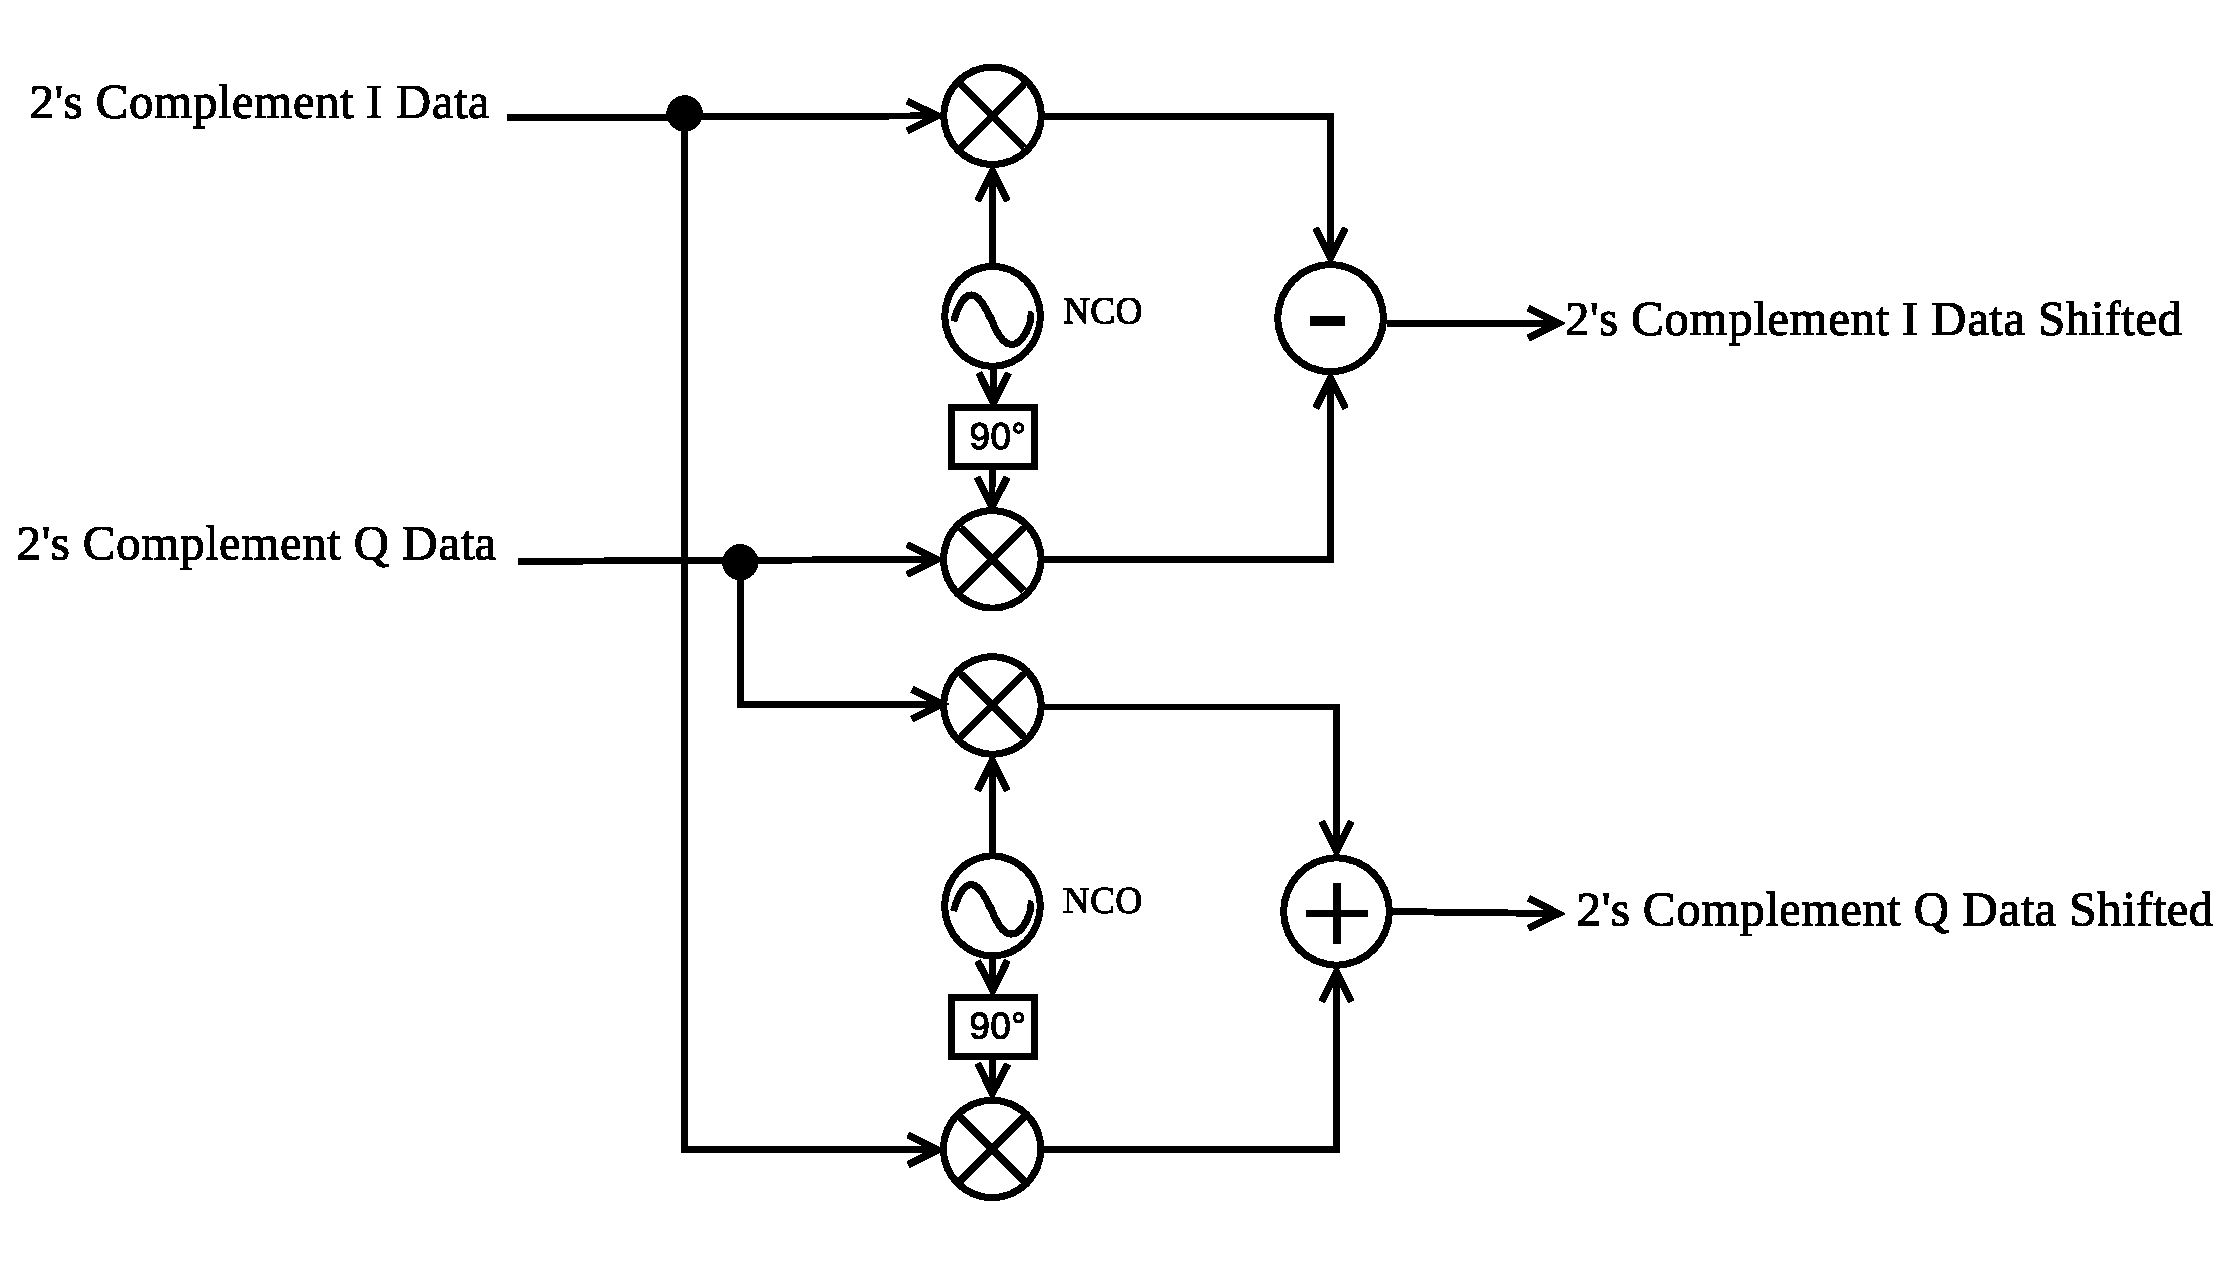
\includegraphics[width=\linewidth]{images/Freq_Shift}
				\caption{Diagram of Arithmetic Operations}
		\end{figure}}
	\end{block}
\end{columns}
\end{frame}

\begin{frame}{\huge Detailed Design} 
\begin{block}{DSP Chain}
	\begin{itemize}
		\item Amplitude Scaling Module
		\begin{itemize}
			\item Received unsigned, time delayed, frequency shifted 32 bit I/Q data 
			\item Received amplitude scaling control word
			\item Applied non circular shifts to get amplitude scale between 1 and $3.05\times 10 ^{-5}$
			\item Did multiplication and checked overflows
		\end{itemize}
	\end{itemize}
	
\end{block}
\end{frame}

\section{Results}
\mode<all>{ 
	\SlideTransition{Results and Conclusions} 
}

\begin{frame}{Results and Conclusions}
	\begin{columns}
				\column{0.5\textwidth}
				\begin{block}{User Interface}
					\action<+->{
						\begin{itemize}
							\item Works well but some latency
							\item Cannot receive data from FGPA
						\end{itemize}
						
					}
				\end{block}
				\begin{block}{Time Delay}
					\action<+->{
						\begin{itemize}
							\item Impossible to see in real time.
						\end{itemize}
						\begin{figure}
							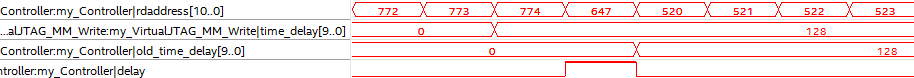
\includegraphics[width =\linewidth]{images/delay}
							\caption{Signal Tap Delay Result}
						\end{figure}
					
						
					}
				\end{block}
				\column{0.5\textwidth}
				\begin{block}{Frequency Shifting}
					\action<+->{
						\begin{itemize}
							\item Injected sum of 5 sinusoids. 
							\item Noise possibly from PWM or from concatenation of vector
						\end{itemize}
						\begin{figure}[h!]
						\centering
						\begin{subfigure}{0.48\linewidth}
							\centering
							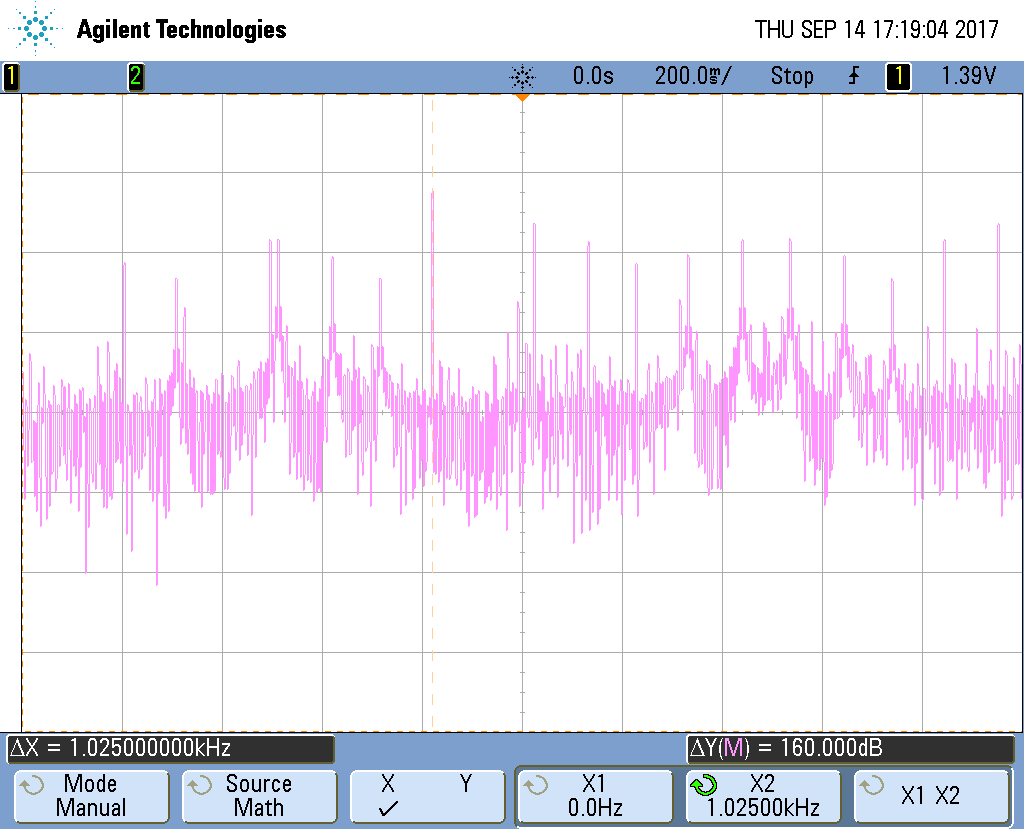
\includegraphics[width=.9\linewidth]{images/scope_3}
							\caption{Oscilloscope Print of a 1kHz frequency shift }
							\label{fig:1khz}
						\end{subfigure}%
						\begin{subfigure}{0.48\linewidth}
							\centering
							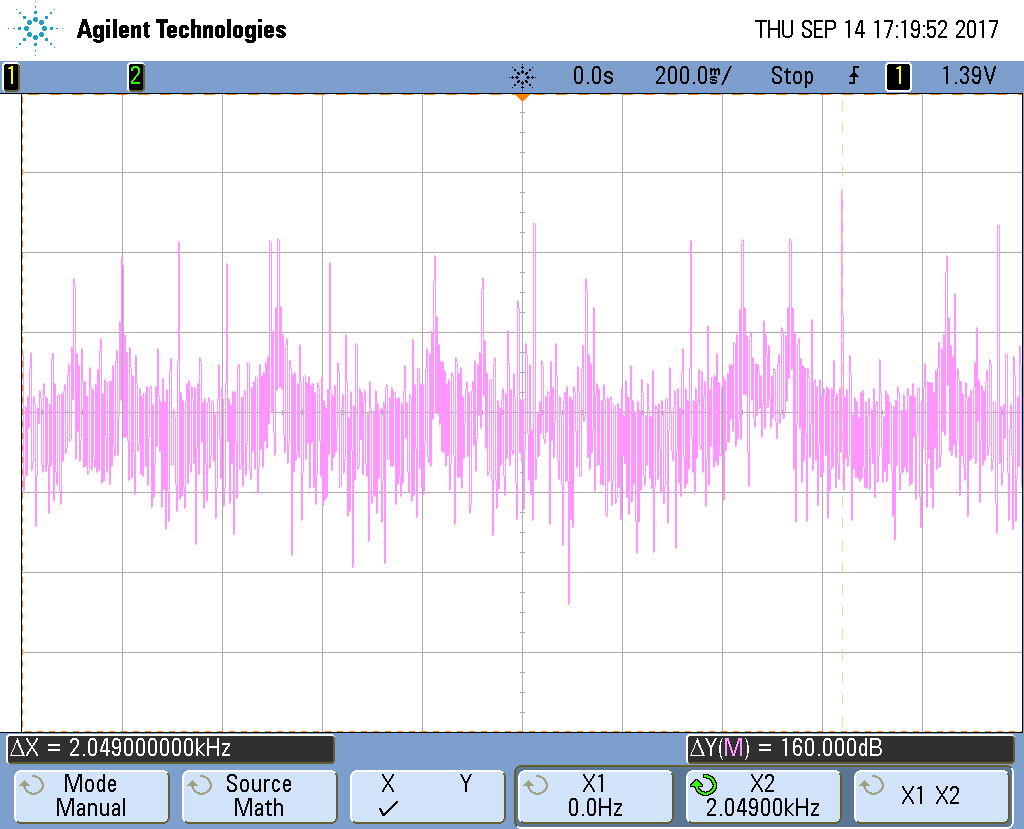
\includegraphics[width=.9\linewidth]{images/scope_4}
							\caption{Oscilloscope Print of a 2kHz frequency shift }
							\label{fig:2khz}
						\end{subfigure}
						\label{fig:2freq}
					\end{figure}
						
					}
				\end{block}
	\end{columns}
\end{frame}

\begin{frame}{Detailed Design}
\begin{columns}
	\column{0.5\textwidth}
	\begin{block}{Frequency Shifting}
		\begin{itemize}
			\item Injected sum of 5 sinusoids. 
			\item Noise possibly from PWM or from concatenation of vector
		\end{itemize}
		\begin{figure}[h!]
			\centering
			\begin{subfigure}{0.48\linewidth}
				\centering
				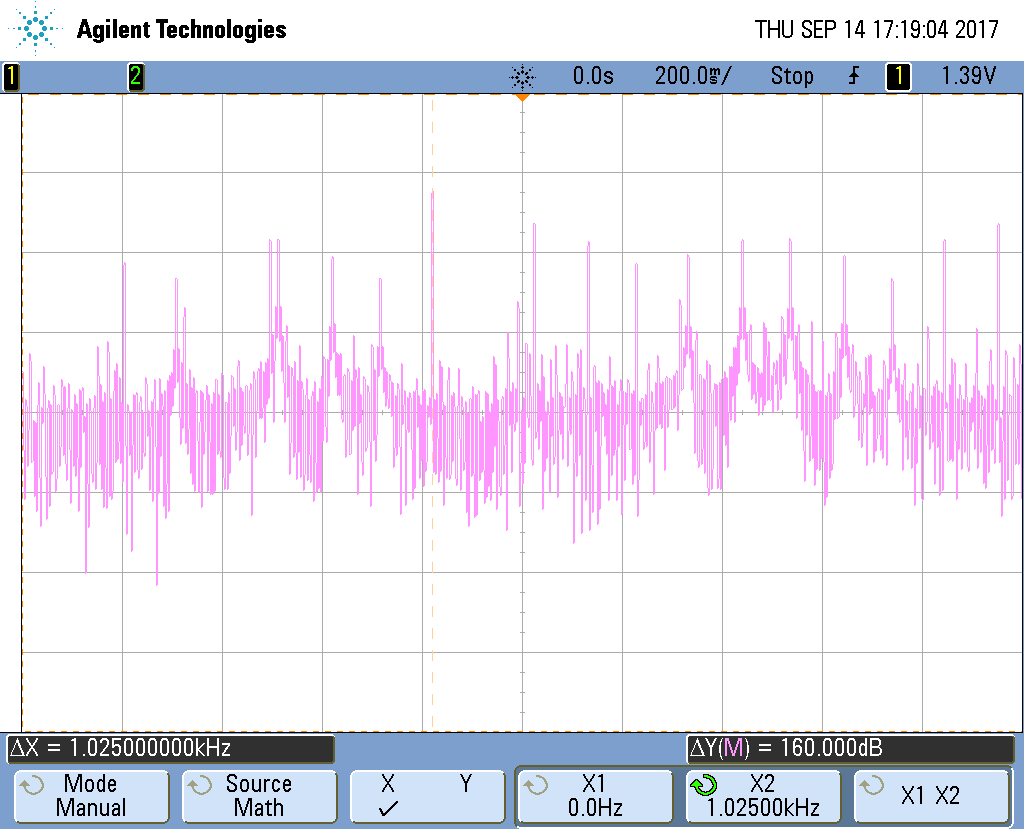
\includegraphics[width=.9\linewidth]{images/scope_3}
				\caption{Oscilloscope Print of a 1kHz frequency shift }
				\label{fig:1khz}
			\end{subfigure}%
			\begin{subfigure}{0.48\linewidth}
				\centering
				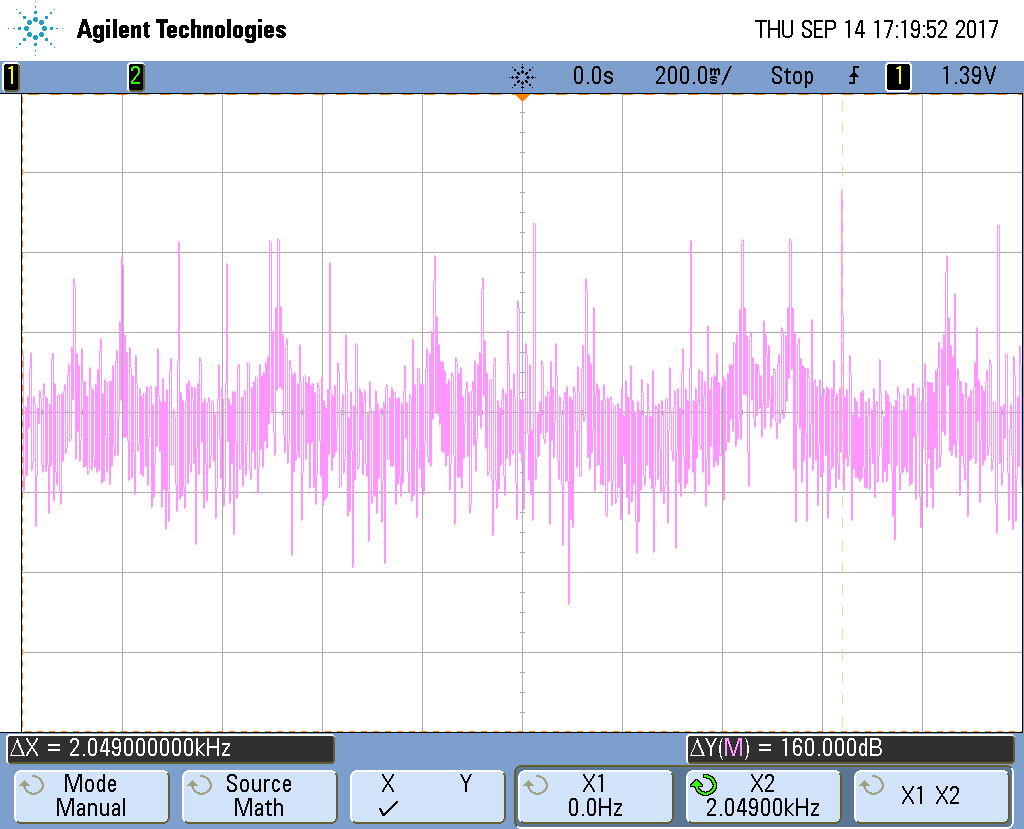
\includegraphics[width=.9\linewidth]{images/scope_4}
				\caption{Oscilloscope Print of a 2kHz frequency shift }
				\label{fig:2khz}
			\end{subfigure}
			\label{fig:2freq}
		\end{figure}
		
	\end{block}
	\column{0.5\textwidth}
	\begin{block}{Amplitude Scaling }<+->
		\action<+->{\begin{itemize}
				\item Very easy to see
				\item Effective.
				\begin{figure}[h!]
					\centering
					\begin{subfigure}[b]{.9\textwidth}
						\centering
						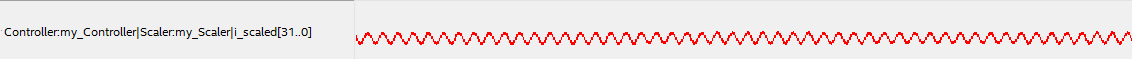
\includegraphics[width=.9\linewidth]{images/full_scale}
						\caption{Full Scale Sinusoid}
						\label{fig:full_scale}
					\end{subfigure}%
					
					
					\begin{subfigure}[b]{.9\textwidth}
						\centering
						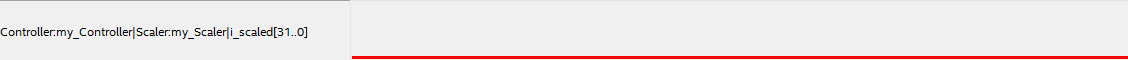
\includegraphics[width=.9\linewidth]{images/attenuated}
						\caption{Fully Attenuated Sinusoid}
						\label{fig:attentuated}
					\end{subfigure}
					\caption{Figures Showing the Measured Amplitude Scaling}
					\label{fig:amp}
				\end{figure}
		\end{itemize}}
	\end{block}
\end{columns}
\end{frame}

\section{Recommendations}
\mode<all>{ 
	\SlideTransition{ Recommendations} 
}
\begin{frame}{Recommendations}
	\begin{block}{Potential Future Work}<+->
		\action<+->{
			\begin{itemize}
					\item Increased Delay Functionality
					\item Improved Frequency Measurement
					\item Integration into a RF Front-end
					\item Extension to Multiple Targets
			\end{itemize}
			}
		
	\end{block}
\end{frame}


\mode<all>{ 
\SlideTransition{Demo} 
}



\mode<all>{ 
\SlideTransition{Questions?}
}


% that's all folks
\end{document}
